\chapter{SPICE Analysis Types, Commands and Options}

\label{chap_spiceanalysistypesparametersandcommands_satco}


The SPICE engine in CoolSPICE is based on ngspice.  The netlist generator creates netlists in the standard SPICE syntax, for which extensive documentation is available online.   The Analysis components in the Schematic Generator are translated into the netlist in the syntax set down here for each analysis type, described here.  As described in Chapter \ref{chap_plotterandnetlisteditor_pane}, these commands can also be directly added to the netlist to run the relevant analyses.

\section{SPICE Suffixes}
\label{subsec_satco_suffixes}
\index{SPICE!suffixes}
These are repeated here for convenience.
\vspace{2\parskip}

\begin{tabular}{lll} 
\textit{suffix} & \textit{name} & \textit{magnitude} \\ \hline \\ \vspace{-0.8\parskip}
a & atto- & $10^{-18}$ \\
f & femto- & $10^{-15}$ \\
p & pico- & $10^{-12}$ \\
n & nano- & $10^{-9}$ \\
u & micro- & $10^{-6}$ \\
m & milli- & $10^{-3}$ \\
k & kilo- & $10^{3}$ \\
meg & mega- & $10^{6}$ \\
g & giga- & $10^{9}$ \\
t & tera- & $10^{12}$ \\
\end{tabular}

\clearpage

\section{Basic SPICE Analysis Types}
\label{sec_satco_basicspiceanalysistypes}

In the syntax statements of this section, parameters are stated with their name between cornered parentheses (\textit{i.e.} \texttt{[]}).  Optional parameters are stated between normal parentheses. 

\subsection{The .SPICE Directive}
\label{sec_satco_thespicedirective}
\index{SPICE directive}
The \textsf{.Spice Directive} component can be used to insert any valid SPICE statement directly into the netlist, including analysis statements.  Figure \ref{fig_spiceanalysis_spicedirectiveexample} shows a \textsf{.dc} statement specified without using the \textsf{.dc} analysis tool (see Section \ref{subsec_satco_dc} below) and how the statement is included in the netlist.

The most important use of this component in CoolSPICE is to define SPICE options by inserting an \texttt{.options} statement.  Section \ref{subsec_satco_spicesimulationoptions} describes the options and their use.

\begin{figure}[b]
  \centering
    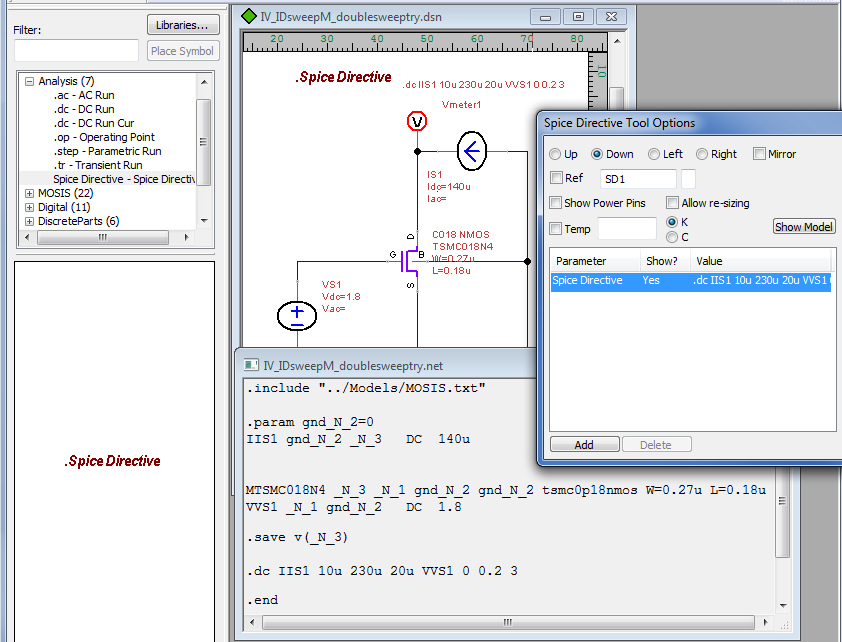
\includegraphics[width=0.8\textwidth]{./figures/spice_analysis_figures/SPICEAnalysis_spicedirective1.png}
    \caption{The analysis component \textsf{.Spice Directive} used to specify a nested DC analysis.}
  \label{fig_spiceanalysis_spicedirectiveexample}
\end{figure} 


\clearpage

\subsection{.ac (AC/Frequency Domain Analysis)}
\label{subsec_satco_ac}

\inserttip{There must be one AC source with a defined value in the circuit for this analysis to run.  However, more than one AC source with defined values can make results hard to interpret.}

\index{SPICE!statements!.ac} 
\index{AC analysis}\index{Frequency domain analysis}
\textbf{\textit{Syntax:}}

\spicesyntax{\begin{tabular}{ll}
.ac dec [POINTSPERDECADE] [START] [END] \\
.ac oct [POINTSPEROCTAVE] [START] [END] \\
.ac lin [POINTS] [START] [END]
\end{tabular}}

\begin{tabular}{lp{5.5cm}p{5cm}}
\textit{parameter} & \textit{description} & \textit{Schematic Editor option}\\ \hline \\ \vspace{-0.8\parskip}
\texttt{[POINTSPERDECADE]} & Number of points within each decade (*) of the frequency range& \textsf{Dec} \\
\texttt{[POINTSPEROCTAVE]} & Number of points within each octave (*) of the frequency range& \textsf{N/A} \\
\texttt{[POINTS]} & Number of points within the frequency range (*) & \textsf{N/A} \\
\texttt{[START]} & Start value for sweep & \textsf{Start Freq} \\
\texttt{[END]} & End value for sweep & \textsf{End Freq} \\
\end{tabular}

\vspace{0.5\parskip}
\inserttip{(*) The AC Run component in the Schematic Editor only implements the decade option; see Remarks below.}
\vspace{0.5\parskip}

\textbf{\textit{Examples:}}

\begin{tabular}{p{5cm}p{8cm}}
\textit{statement} & \textit{explanation} \\ \hline \\ \vspace{-0.8\parskip} 
\texttt{.ac dec 30 10k 100meg} & {\small Sweep the AC source frequency from 10 kHz to 100 MHz, 30 points per decade} \\
\texttt{.ac lin 20 10meg 20meg} & {\small Sweep the AC source frequency from 10 MHz to 20 MHz in 20 points} \\
\texttt{.ac oct 16 2meg 64meg} & {\small Sweep the AC source frequency from 2 MHz to 64 MHz in 16 points per octave} \\
\end{tabular}

\textbf{\textit{Remarks: Linear and Per Octave Point Separation}}

The AC Run component in the Schematic Editor only implements the points-per-decade option.  The user can implement linearly spaced points or the points-per-octave option with the syntax shown here by using the Netlist Editor.

Further options for an AC simulation can be set through an \texttt{.options} statement as described in Section \ref{subsec_satco_acoptions}.
\newpage

\subsection{.dc (DC Analysis)}
\label{subsec_satco_dc}

\index{SPICE!statements!.dc}\index{DC analysis}
\textbf{\textit{Syntax:}}

\spicesyntax{\begin{tabular}{ll}
.dc & [SOURCENAME] [START] [END] [INCREMENT] \\
& ([SOURCENAME 2] [START 2] [END 2] [INCREMENT 2])
\end{tabular}
}

\begin{tabular}{lp{5.5cm}p{5cm}}
\textit{parameter} & \textit{description} & \textit{Schematic Editor option}\\ \hline \\ \vspace{-0.8\parskip}
\texttt{[SOURCENAME]} & Reference name of the source whose DC value is swept \textbf{(*)} & \textsf{Voltage Source1/\newline Current Source1}\\
\texttt{[START]} & Start value for sweep & \textsf{V1start/I1start} \\
\texttt{[END]} & End value for sweep & \textsf{V1end/I1end} \\
\texttt{[INCREMENT]} & Step size for sweep & \textsf{V1step/I1step} \\
\texttt{[SOURCENAME 2]} & Reference name of the {second source for DC sweep \textbf{(*)}} & \textsf{Voltage Source2/\newline Current Source2}\\
\texttt{[START 2]} & Start value for second sweep & \textsf{V1start/I1start} \\
\texttt{[END 2]} & End value for second sweep & \textsf{V1end/I1end} \\
\texttt{[INCREMENT 2]} & Step size for second sweep & \textsf{V1step/I1step} \\
\end{tabular}

\vspace{0.5\parskip}
\inserttip{(*) The netlister adds a \texttt{"V"} before the Reference Name set in the \window{Options} for a voltage source and a \texttt{"I"} for a current source.  \textit{E.g.} a DC voltage source \textsf{VGATE} has the name \texttt{VVGATE} in the SPICE statement.  The SOURCENAME parameter \textit{must} have the name as it is in the SPICE statement, i.e. \texttt{VVGATE} for this example, \textit{not} \texttt{VGATE}.}
\vspace{0.5\parskip}

\textbf{\textit{Examples:}}

\begin{tabular}{p{5cm}p{8cm}}
\textit{statement} & \textit{explanation} \\ \hline \\ \vspace{-0.8\parskip} 
\texttt{.dc IIS1 10u 230u 10u} & {\small Sweep the DC current source \textsf{``IIS1"} \textbf{(*)} from 10 $\mu$A to 230 $\mu$A in steps of 10 $\mu$A} \\
\texttt{.dc VVS1 0 30 0.1} & {\small Sweep the DC voltage source \textsf{``VVS1"} from 0 V to 30 V in steps of 0.1 V} \\
\texttt{.dc IIS1 10u 230u 10u \newline +VVS1 0 3 0.5} & {\small Step the DC voltage source \textsf{``VVS1"} from 0 V to 3 V in steps of 0.5 V; at each step sweep the DC current source \textsf{``IIS1"} from 10 $\mu$A to 230 $\mu$A in steps of 10 $\mu$A} {(**)}
\end{tabular}

\inserttip{(*) The source names in all examples here are as in the SPICE statements, not as in the Reference Name boxes; see note above.   (**) This statement can only be set in the netlist, not from the Schematic Editor.  See ``Nested Sweeps" below.}

\textbf{\textit{Remarks: Nested Sweeps}}
\index{DC analysis!nested sweeps}

Nested sweeps of two voltage sources can be set from the Schematic Editor by specifying both sweeps in the DC Run component.  Similarly, nested sweeps of two current sources can be set by specifying both in the DC Run Current component.  However, it is not possible to use a component in the Schematic Editor to set a nested voltage/current or current/voltage sweep.  A SPICE statement such as the last example given above has to be entered into the netlist for that purpose.

Further options for a DC simulation can be set through an \texttt{.options} statement as described in Section \ref{subsec_satco_dcoptions}.

\subsection{.op (Operating Point)}
\label{subsec_satco_op}

\index{SPICE!statements!.op}
\textbf{\textit{Syntax:}}

\spicesyntax{\begin{tabular}{ll}
.op&
\end{tabular}
}

\textbf{\textit{Remarks:}}

Capacitors are considered open circuit and inductors are considered as closed circuit for the operating point analysis.

The operating point analysis results can be seen in the rawfile by using \menuorbutton{SPICE}$\to$\menuorbutton{Preferences}$\to$\menuorbutton{Show Rawfile}.  If the \menuitem{SPICE}{Run OP Analysis} is used, the program will run the operating point analysis and display the results near the meter components in the drawing, but the \textsf{.op} command will not be included in the netlist when it is generated unless the \textsf{.op} component from the \textsf{Analysis} menu is used.

\subsection{.step (Parametric Analysis)}
\label{subsec_satco_step}

%\askakin{In the ngspice manual, this is mentioned only on pages 269 and 270, \\
%as a control loop that is described to "replace .STEP".  \\
%Did you reinstate its implementation?}

\index{SPICE!statements!.step}\index{Parametric sweeps}
\inserttip{The \texttt{.step} command is not, in itself, an analysis command.  It is used in conjunction with another analysis command such as \texttt{.op} to run through that analysis multiple times. }

\textbf{\textit{Syntax:}}

\spicesyntax{\begin{tabular}{ll}
.step & [PARAMNAME] [START] [END] [INCREMENT] 
\end{tabular}}

\begin{tabular}{lp{5.5cm}p{5cm}}
\textit{parameter} & \textit{description} & \textit{\textsf{Schematic Editor} option}\\ \hline \\ \vspace{-0.8\parskip}
\texttt{[PARAMNAME]} & \textit{Component Value} to sweep \textbf{(*)} & \textsf{Parameter}\\
\texttt{[START]} & Start value for sweep & \textsf{Start} \\
\texttt{[END]} & End value for sweep & \textsf{End} \\
\texttt{[INCREMENT]} & Step size for sweep & \textsf{Step}
\end{tabular}

\inserttip{(*) To run a parametric sweep, the value of a component parameter must be defined as a parameter name instead of a numerical value.  [PARAMNAME] in the \texttt{.step} statement must then be the same.  See Fig. \ref{fig_spiceanalysis_paramexample} for an example.}

\begin{SCfigure}[5.0][hbt]
    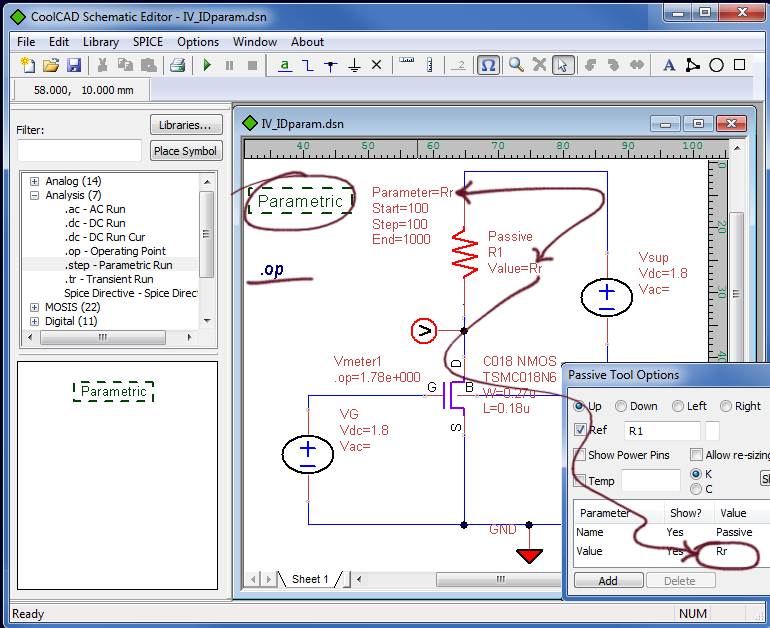
\includegraphics[width=0.65\textwidth]{./figures/spice_analysis_figures/SPICEAnalysis_parametric1.png}
    \caption{{The transistor circuit operating point is evaluated by changing the value of the resistor connected to the drain from \mbox{100 $\Omega$} to 1000 $\Omega$ in 100 $\Omega$ steps.}}
  \label{fig_spiceanalysis_paramexample}
\end{SCfigure}

\subsection{.tran (Transient Analysis)}
\label{subsec_satco_tran}

\index{SPICE!statements!.tran}\index{Transient analysis}
\spicesyntax{\begin{tabular}{ll}
.tran & [STEP] [END] ([START] [MAXSTEP] [UIC])
\end{tabular}
}

\begin{tabular}{lp{5.5cm}p{5cm}}
\textit{parameter} & \textit{description} & \textit{Schematic Editor option}\\ \hline \\ \vspace{-0.8\parskip}
\texttt{[STEP]} & Time step size for {storing results} \textbf{(*)} & \textsf{Time Step}\\
\texttt{[END]} & Stop time for simulation & \textsf{End Time} \\
\texttt{[START]} & Start time for simulation & \textsf{Start Time} \\
\texttt{[MAXSTEP]} & Maximum time step in the adaptive transient simulation & \textsf{Max Step} \\
\texttt{[UIC]} & "Use initial conditions" (*) & \textsf{N/A} 
\end{tabular}

\inserttip{(*) The \textsf{.tran} component in the Schematic Editor does not include a way to specify this option.  It should be specified in the netlist by using the Netlist Editor if desired.}

\textbf{\textit{Examples:}}

\begin{tabular}{p{5cm}p{8cm}}
\textit{statement} & \textit{explanation} \\ \hline \\ \vspace{-0.8\parskip} 
\texttt{.tran 10n 100u} & {\small Run a transient simulation from $t$=0 to \newline $t=100\mu$s, store the results every 10 ns} \\
\texttt{.tran 10n 100u 0 5n} & {\small Run a transient simulation from $t$=0 to \newline $t=100\mu$s with a maximum time step of 5 ns, store the results every 10 ns} \\
\texttt{.tran 10n 100u 50u 5n} & {\small Run a transient simulation from $t$=0 to \newline $t=100\mu$s with a maximum time step of 5 ns, store the results every 10 ns \newline starting from $t=50\mu$s} \\
\texttt{.tran 10n 80u uic} & {\small Run a transient simulation from $t$=0 to \newline $t=80\mu$s, do not calculate the quiescent operating point beforehand}
\end{tabular}

\textbf{\textit{Remarks:}}

If ``\texttt{uic}" is specified at the end of the \texttt{.tran} statement, the simulator will not solve for the quiescent operating point before the transient analysis. If there are IC values specified on elements, CoolSPICE will use these values (see Section \ref{sec_satco_initialconditions}).  If there are none, all node voltages will be assumed to be zero initially.  This may lead to problems.

Further options for a transient simulation can be set through an \texttt{.options} statement as described in Section \ref{subsec_satco_tranoptions}.

\section{Initial Conditions}
\label{sec_satco_initialconditions}

\index{Initial conditions}
There are two ways of specifying initial conditions within CoolSPICE:

\begin{itemize}
\item  The \textsf{IC - Initial Condition} tool in the \textsf{Analog} library.  This allows the user to set an initial condition voltage at a given node and corresponds to a \textsf{.ic} statement in the netlist.  
\item Initial conditions can be set for voltages across capacitors and currents across inductors by editing the device statements in the netlist.  
\end{itemize}

This section describes the first method.

\subsection{The \texttt{.ic} Statement}
\label{sec_satco_icstatement}

\index{SPICE!statements!.ic}
\textbf{\textit{Syntax:}}

\spicesyntax{\begin{tabular}{ll}
.ic & v([NODELABEL])=[VALUE]
\end{tabular}}

\begin{tabular}{lp{5.5cm}p{5cm}}
\textit{parameter} & \textit{description} & \textit{Schematic Editor option}\\ \hline \\ \vspace{-0.8\parskip}
\texttt{[NODELABEL]} & Name or label of the node at which the IC is set & \textsf{N/A, graphical} \\
\texttt{[VALUE]} & The initial condition value & \textsf{N/A} 
\end{tabular}

\textbf{\textit{Examples:}}

\begin{tabular}{p{5cm}p{8cm}}
\textit{statement} & \textit{explanation} \\ \hline \\ \vspace{-0.8\parskip} 
\texttt{.ic v(Vin)=2} & {\small Set the initial condition on node connected to the wire labeled \texttt{Vin} to 2 V} \\
\texttt{.ic v(\_N\_6)=0.5} & {\small Set the IC on the {automatically-named node \texttt{\_N\_6}} to 0.5 V}
\end{tabular}

\section{The \texttt{.meas} Statement}
\label{sec_satco_measstatement}


The \texttt{.meas} (or \texttt{.measure}) statement is used to take measurements (such as a signal period) on the simulation output data after a simulation is successfully completed.  This is a very versatile and powerful statement which serves many of the same purposes as taking measurements on a plotted result after the simulation, but yields results much faster and without user intervention or the need to use a graphical plot.  It can be used to measure results from \texttt{.ac}, \texttt{.dc} or \texttt{.tran} statements.  

\texttt{.measure} statements can be used to measure times elapsed between trigger voltage levels (e.g. period of a periodic signal, or rise/fall/delay times), to measure average, RMS, minimum or maximum values, or values or times when a specific event such as two signals crossing each other occurs.  This section of the  manual will be expanded in the next edition to describe the full use of the statement.  

The example file \textsf{Meas\_example.dsn} under the \textsf{Ckts/} folder in the default CoolSPICE installation shows the \textsf{.measure} command being used.  Note that in the Schematic Editor, the \texttt{.meas} statement is specified using the \textsf{.Spice Directive} component.  To use this method, the \textsf{Measure} option must be checked under the \menuitem{SPICE}{Preferences}.  No rawfile is saved during such a run and the Plotter will not be invoked even if the option is set to open it automatically after a simulation.  

% \textbf{\textit{Syntax:}}

% \spicesyntax{\begin{tabular}{ll}
% .meas & [MEASUREMENTTYPE] [DATA] [POSITIONID] [POSITIONVARIABLE]=[VALUE] \\
% & TD/AT=[TDORATVALUE] CROSS/RISE/FALL=[CROSSRISEFALLVALUE] TARG [MARKERVARIABLE] 
% \end{tabular}}

\section{The \texttt{.param} Statement}
\label{sec_satco_paramstatement}

\index{SPICE!statements!.param}\index{SPICE!defining parameters}\index{Parameters}
With the \texttt{.param} statement, the user can define constants or numerical values for an alphanumeric identifier, which can then be referred to throughout the rest of the circuit definition.    This option is not available directly through the Schematic Editor (except when using a \texttt{.step} analysis; see below) but can be easily used through the Netlist Editor. 

\textbf{\textit{Syntax:}}

\spicesyntax{\begin{tabular}{ll}
.param & [IDENTIFIER1]=[VALUE1] ([IDENTIFIER2]=[VALUE2]) (...)
\end{tabular}}

\begin{tabular}{lp{5.5cm}p{5cm}}
\textit{parameter} & \textit{description} & \textit{Schematic Editor option}\\ \hline \\ \vspace{-0.8\parskip}
\texttt{[IDENTIFIER]} & Name for the identifier & \textsf{N/A (*)} \\
\texttt{[VALUE]} & The value or constant & \textsf{N/A (*)} 
\end{tabular}

\inserttip{(*) When a \texttt{.step} analysis is being used to step through a range of values for a component, it is possible to set the value of the component to a parameter.  In that case, the netlister will insert a \texttt{.param} statement into the netlist and set its value to the start value of the \texttt{.step} statement.  Figure \ref{fig_spiceanalysis_paramexample} shows an example case, for which the netlister will include the line {\texttt{.param Rr=100}} in the netlist.}

\textbf{\textit{Examples:}}

\begin{tabular}{p{5cm}p{8cm}}
\textit{statement} & \textit{explanation} \\ \hline \\ \vspace{-0.8\parskip} 
\texttt{.param pi=3.1415} & {\small Set \texttt{``pi"} to 3.1415.} \\
\texttt{.param Rd=200} & {\small Define \texttt{Rd} as 200 $\Omega$, to later refer to it in 
lines such as {\texttt{Rdrain1 D1 VDD\_n Rd}} and \newline \nobreak{{\texttt{Rdrain45 D45 VDD\_n Rd}}}.}
\end{tabular}

\textbf{\textit{Remarks:}}

The first character of the identifier must be alphabetic.  The rest can be alphanumeric and use the  \texttt{! \# \$ \% [ ] \_} characters. The following words are reserved keywords in SPICE and must not be used as parameter names: \texttt{abs}, \texttt{and}, \texttt{arctan}, \texttt{cos}, \texttt{defined}, \texttt{div}, \texttt{exp}, \texttt{hertz}, \texttt{ln}, \texttt{mod}, \texttt{not}, \texttt{or}, \texttt{pwr}, \texttt{sin}, \texttt{sqr}, \texttt{sqrt}, \texttt{temper}, \texttt{time}.

\subsection{\texttt{.param} Functions}

A number of functions are available for use in conjunction with .param statements.

\begin{longtable}{c c}

\hline\hline %inserts double horizontal lines
Function Name & Description \\ [0.5ex] % inserts table
%heading
\hline % inserts single horizontal line
abs(x) & Absolute value of x \\ \\ % inserting body of the table

agauss(nom, avar, sigma) & \begin{minipage}{20em}
  Nominal value plus variation drawn from Gaussian distribution 
	with mean 0 and standard deviation absolute value of avar, divided by sigma
\end{minipage}\\ \\

arcsin(x), asin(x), arccos(x),\\ 
acos(x), arctan(x), atan(x), & \begin{minipage}{20em}
Inverse trigonometric functions. Note these functions give the real part only.
\end{minipage}\\ \\

asinh(x), acosh(x), atanh(x) & \begin{minipage}{20em}
Inverse hyperbolic trigonometric functions. Note these functions give the real part only.
\end{minipage}\\ \\

atan2(y, x) & \begin{minipage}{20em}
Fourth quadrant inverse tangent of y$/$x
\end{minipage}\\ \\

buf(x) & \begin{minipage}{20em}
(x$>$0.5) ? 1.0 : 0.0
\end{minipage}\\ \\

cbrt(x) & \begin{minipage}{20em}
Cube root of x
\end{minipage}\\ \\

ceil(x) & \begin{minipage}{20em}
Smallest integer that is greater than or equal to x
\end{minipage}\\ \\

defined(symbol) & \begin{minipage}{20em}
1 if symbol is defined, else 0
\end{minipage}\\ \\

exp(x) & \begin{minipage}{20em}
e$\rm{^x}$
\end{minipage}\\ \\

flat(x) & \begin{minipage}{20em}
Randomly generated number between -x and x with uniform distribution
\end{minipage}\\ \\

floor(x), int(x) & \begin{minipage}{20em}
Largest integer that is less than or equal to x
\end{minipage}\\ \\

gauss(nom, rvar, sigma) & \begin{minipage}{20em}
Nominal value plus variation drawn from Gaussian distribution with mean 0 and standard deviation rvar (relative to nominal, divided by sigma
\end{minipage}\\ \\

hypot(x, y) & \begin{minipage}{20em}
sqrt((x$\rm{^2}$) + (y$\rm{^2}$))
\end{minipage}\\ \\

inv(x) & \begin{minipage}{20em}
(x$>$0.5) ? 0.0 : 1.0
\end{minipage}\\ \\

limit(nom, avar) & \begin{minipage}{20em}
Nominal value $\pm$ avar, depending on random number in [-1, 1] being $>$ 0 or $<$ 0
\end{minipage}\\ \\

ln(x), log(x) & \begin{minipage}{20em}
Natural log of x
\end{minipage}\\ \\

max(x, y) & \begin{minipage}{20em}
x $>$ y ? x : y
\end{minipage}\\ \\

mc(x, y) & \begin{minipage}{20em}
Randomly generated real number y such that  x$\cdot$(1-y) $<$ y $<$ x$\cdot$(1+y) with uniform distribution
\end{minipage}\\ \\

min(x, y) & \begin{minipage}{20em}
x $<$ y ? x : y
\end{minipage}\\ \\

nint(x), round(x) & \begin{minipage}{20em}
Round to nearest int, x.5 rounds to x+1.
\end{minipage}\\ \\

pow(x, y) & \begin{minipage}{20em}
x raised to the power of y (pow from C runtime library)
\end{minipage}\\ \\

pwr(x, y) & \begin{minipage}{20em}
pow(fabs(x),y), note that this function gives only the real part of the answer
\end{minipage}\\ \\

pwrs(x, y) & \begin{minipage}{20em}
sgn(x)$\cdot$abs(x)$\rm{^y}$
\end{minipage}\\ \\

rand(x), random(x) & \begin{minipage}{20em}
Randomly generated real number y such that 0 $<$ y $<$ 1 depending on the integer value of x
\end{minipage}\\ \\

sgn(x) & \begin{minipage}{20em}
1.0 for x $>$ 0, 0.0 for x equal to 0, -1.0 for x $<$ 0 
\end{minipage}\\ \\

sin(x), cos(x), tan(x) & \begin{minipage}{20em}
Trigonometric functions
\end{minipage}\\ \\

sinh(x), cos(x), tanh(x) & \begin{minipage}{20em}
Hyperbolic trigonometric functions
\end{minipage}\\ \\

sqr(x) & \begin{minipage}{20em}
y=x$\rm{^2}$
\end{minipage}\\ \\

sqrt(x) & \begin{minipage}{20em}
y=$\sqrt{\rm{x}}$, note that this function gives only the real part of the answer
\end{minipage}\\ \\

table(x, $\rm{x_1,y_1, x_2,y_2}$, ... ) & \begin{minipage}{20em}
Piecewise linear function where the answer value y, is interpolated base on the pair of points between which x falls.
\end{minipage}\\ \\

ternary\_fcn(x, y, z), if(x, y, z) & \begin{minipage}{20em}
x ? y : z
\end{minipage}\\ \\

u(x) & \begin{minipage}{20em}
Unit step, x $>$ 0 ? 1 : 0
\end{minipage}\\ \\

unif(nom, rvar) & \begin{minipage}{20em}
Nominal value plus relative variation (to nominal) uniformly distributed between $\pm$rvar
\end{minipage}\\ \\

uramp(x) & \begin{minipage}{20em}
x $>$ 0 ? x : 0
\end{minipage}\\ \\[1ex] % [1ex] adds vertical space
\hline %inserts single line

\caption{.param functions}
\label {tab:paramfuncs}
\end{longtable}

\section{The \texttt{.save} Statement}
\label{subsec_satco_savestatement}

\index{SPICE!statements!.save}
The \texttt{.save} statement is used to save node voltage and branch current values in the output rawfile. The Plotter can display these values as traces. The netlister automatically inserts the relevant \texttt{.save} statements in the netlist when the components \textsf{Probe - Ammeter} and \textsf{Probe - Voltmeter} from the \textsf{Analog} library are used in the Schematic Editor (see Section \ref{subsec_se_probes}).  

\inserttip{Note that it is only possible to save the current through an independent voltage source.  The current probe component in the Schematic Editor is actually a zero-volt DC source.}

\textbf{\textit{Syntax:}}

\spicesyntax{\begin{tabular}{ll}
.save & v([NODELABEL]) \\
.save & i([VOLTAGESOURCEREF])
\end{tabular}}

\begin{tabular}{lp{5.5cm}p{5cm}}
\textit{parameter} & \textit{description} & \textit{Schematic Editor option}\\ \hline \\ \vspace{-0.8\parskip}
\texttt{[NODELABEL]} & The label or name of a node in the circuit. & \textsf{N/A} \\
\texttt{[VOLTAGESOURCEREF]} & {The Reference Name of a voltage source or a current probe, prefixed with a ``\texttt{V}" if taken from the Schematic Editor Options (*)} & \textsf{Ref} (*) 
\end{tabular}

\inserttip{(*) The netlister will prefix the reference name of a voltage source or current probe with ``\texttt{V}".  For instance, a DC voltage source whose reference name is set as ``V\_DS" and a current probe whose reference name is set as ``Imeter1" in the \window{Options} will appear as ``\texttt{VV\_DS}" and ``\texttt{VImeter1}" in the netlist respectively.  The \texttt[VOLTAGESOURCEREF] parameter in the \texttt{.save} statement must be in this prefixed form.}

\textbf{\textit{Examples:}}

\begin{tabular}{p{5cm}p{8cm}}
\textit{statement} & \textit{explanation} \\ \hline \\ \vspace{-0.8\parskip} 
\texttt{.save v(\_N\_6)} & {\small Save the voltage at the node ``\texttt{\_N\_6}" }\\
\texttt{.save v(diffampout)} & {\small Save the voltage at the line labeled ``\texttt{diffampout}," which corresponds to a node.} \\
\texttt{.save i(VDS1)} & {\small Save the current through the voltage source \texttt{VDS1}, which will have the reference name as ``DS1" in the \window{Options} if defined through the Schematic Editor.}
\end{tabular}

\section{SPICE Simulation Options}
\label{subsec_satco_spicesimulationoptions}

%(The \textsf{.options} statement)
\index{SPICE!statements!.options}\index{SPICE!simulator options}\index{Options}
SPICE simulation options can be set through the \texttt{.options} statement, which has to be entered in the netlist through the Netlist Editor.  Multiple options can be entered in a single statement.  

\textbf{\textit{Syntax:}}

\spicesyntax{\begin{tabular}{ll}
.options [OPTION1] [OPTION2] [...] \\
.options [OPTION1]=[VALUE] [OPTION2]=[VALUE] 
\end{tabular}}

In the tables of this section, options which are toggled on- or off- just have names listed, while options which should have a value set are shown with an ``equal" sign (\textit{e.g.} \texttt{ABSTOL=}).

\subsection{General Options}
\label{subsec_satco_generaloptions}

\begin{tabular}{lp{8cm}p{2cm}}
\textit{option} & \textit{description} & \textit{default value}\\ \hline \\ \vspace{-0.8\parskip}
\texttt{ACCT} & Print runtime statistics & On \\
\texttt{NOACCT} & Do not print runtime statistics or the initial transient solution & Off \\
\texttt{NOINIT} & Do not print the initial transient solution & Off \\
%\texttt{[LIST]} & Print the summary listing of the input data & \textsf{N/A} \\ NOT SURE IF WORKS
%\texttt{[NOMOD]} & Do not print the model parameters & \textsf{N/A} \\
% \texttt{[NODE]} & Print the node table & \textsf{N/A} \\ SEEMS NOT TO WORK
%\texttt{[OPTS]} & Print the option values & \textsf{N/A} \\
\texttt{TEMP=} & Circuit operating temperature; can be overridden on devices & $27\,^{\circ}\mathrm{C}$ \\
\texttt{TNOM=} & Nominal temperature for device parameter measurements & $27\,^{\circ}\mathrm{C}$
%\texttt{[WARN]} & I'm not sure if WARN  and MAXWARN work or not
\end{tabular}

All the options about printing/not printing certain outputs pertain to the \textsf{.log} file created after the simulation.  The log file is by default written in the same directory as the design (\textsf{.dsn}) file and shares the file name.  The log file display can be invoked automatically after each simulation by using the \menuitem{SPICE}{Preferences} of the Schematic Editor.

\subsection{DC Simulation Options}
\label{subsec_satco_dcoptions}

\begin{tabular}{p{2cm}|lp{8cm}p{1.5cm}}
\textit{type} &\textit{option} & \textit{description} & \textit{default value}\\ \hline \\ \vspace{-0.8\parskip}
{{\footnotesize Error tolerance}} & & & \\
&\texttt{ABSTOL=} & Limit for the absolute current error tolerance & 1 pA \\
&\texttt{RELTOL=} & Relative error tolerance & 0.001  \\
&\texttt{VNTOL=} & Limit for the absolute voltage error tolerance & 1 mV  \\
{{\footnotesize Ensuring convergence}} & & & \\
&\texttt{GMIN=} & Minimum conductance allowed & 1e-12 \\
&\texttt{ITL1=} & DC solution number of iterations limit & 100  \\
&\texttt{ITL2=} & DC transfer curve number of iterations limit & 50  \\
&\texttt{PIVREL=} & Ratio between the largest value in a column and the acceptable pivot value & 1e-3  \\
&\texttt{PIVTOL=} & The smallest acceptable pivot value & 1e-13  \\
&\texttt{RSHUNT=} & Value for a resistor to be inserted between each node and the ground & N/A  \\
{\footnotesize Other} & & & \\
&\texttt{KEEPOPINFO} & Retain OP analysis information for AC analyses & Off 
\end{tabular}


\subsection{AC Simulation Options}
\label{subsec_satco_acoptions}

\begin{tabular}{p{2cm}|lp{8cm}p{1.5cm}}
&\textit{option} & \textit{description} & \textit{default value}\\ \hline \\ \vspace{-0.8\parskip}
&\texttt{NOOPAC} & Do not perform the OP analysis before the AC analysis (Invalid if there are nonlinear elements in the circuit) & \\
\end{tabular}

\subsection{Transient Simulation Options}
\label{subsec_satco_tranoptions}

\begin{tabular}{p{2cm}|lp{8cm}p{1.5cm}}
\textit{type} &\textit{option} & \textit{description} & \textit{default value}\\ \hline \\ \vspace{-0.8\parskip}
{{\footnotesize Error tolerance}} & & & \\
&\texttt{CHGTOL=} & Limit for the charge tolerance & 1e-14 \\
&\texttt{TRTOL=} & Transient error tolerance & 7  \\
{{\footnotesize Ensuring convergence}} & & & \\
&\texttt{GMINSTEPS=} & Number of gmin steps to be attempted & 1 \\
&\texttt{ITL3=} & Lower limit for iteration & 4  \\
&\texttt{ITL4=} & Time-point iteration limit & 10  \\
&\texttt{ITL5=} & Total iteration limit & 5000  \\
&\texttt{ITL6=} & (See \texttt{SRCSTEPS}) &   \\
&\texttt{RAMPTIME=} & Rate of change for independent supplies and passives with ICs &   \\
&\texttt{SRCSTEPS=} & (If set to non-zero) Use a source-stepping method to solve for the OP & 0  \\
{\footnotesize Integration} & & & \\
&\texttt{MAXORD=} & Maximum order for the {numerical integration method (see \texttt{METHOD}).} (*) & 2  \\
&\texttt{METHOD=} & The numerical integration method (gear or trapezoidal) & trap  \\
{\footnotesize Other} & & & \\
&\texttt{AUTOSTOP} & Stop the analysis after all .meas commands have been executed (see Section \ref{sec_satco_measstatement}) & Off 
\end{tabular}

\subsection{Element-Specific Options}
\label{subsec_satco_specoptions}

\inserttip{These options will not affect the device \textit{models}, but only the device \textit{instances}.  The relevant option has to be set in the device line in the netlist for the reset or scale values here to be effective. If these are set in an \texttt{.options} line, they override the relevant parameter in all devices.}

\begin{tabular}{p{2cm}|lp{8cm}p{1.5cm}}
&\textit{option} & \textit{description} & \textit{default value}\\ \hline \\ \vspace{-0.8\parskip}
&\texttt{DEFAD=} & Define \texttt{AD}, the MOS drain diffusion area & 0.0 \\
&\texttt{DEFAS=} & Define \texttt{AS}, the MOS source diffusion area & 0.0 \\
&\texttt{DEFL=} & Define \texttt{L}, the MOS channel length & 100 $\mu$m \\
&\texttt{DEFW=} & Define \texttt{W}, the MOS channel width & 100 $\mu$m \\
&\texttt{SCALE=} & Element scaling factor for dimensional parameters with a default unit of meters (*) & 1 \\
&\texttt{TRYTOCOMPACT} & (Applies only to transmission lines using the \texttt{LTRA} model) Attempt to condense past input voltage/current history. & OFF 
\end{tabular}

\textbf{(*)} This applies to MOSFET parameters \texttt{AD, AS, L, PD, PS, SA, SB, SC, SD} and \texttt{W}, to diode parameters \texttt{Area, W, L}, to resistor and capacitor parameters \texttt{L} and \texttt{W}, and to JFET/MESFET parameters \texttt{Area, W} and \texttt{L}.  If, for instance, a MOSFET length is defined as \texttt{L=2.5} and the line \texttt{.options SCALE=1u} is given, the MOSFET length in simulation will be 2.5 $\mu$m.




\begin{enumerate}
\index{ngspice!website}
\item NGSPICE: Mixed Mode - Mixed Level Circuit Simulator, http://ngspice.sourceforge.net, last visited October 2014.

\index{spice!analysis statements}
\item List of SPICE statements, http://www.ecircuitcenter.com/SPICEsummary.htm\#statements, last visited October 2014.

\end{enumerate} 

